% 
% Annual Cognitive Science Conference
% Sample LaTeX Paper -- Proceedings Format
% 

% Original : Ashwin Ram (ashwin@cc.gatech.edu)       04/01/1994
% Modified : Johanna Moore (jmoore@cs.pitt.edu)      03/17/1995
% Modified : David Noelle (noelle@ucsd.edu)          03/15/1996
% Modified : Pat Langley (langley@cs.stanford.edu)   01/26/1997
% Latex2e corrections by Ramin Charles Nakisa        01/28/1997 
% Modified : Tina Eliassi-Rad (eliassi@cs.wisc.edu)  01/31/1998
% Modified : Trisha Yannuzzi (trisha@ircs.upenn.edu) 12/28/1999 (in process)
% Modified : Mary Ellen Foster (M.E.Foster@ed.ac.uk) 12/11/2000
% Modified : Ken Forbus                              01/23/2004
% Modified : Eli M. Silk (esilk@pitt.edu)            05/24/2005
% Modified : Niels Taatgen (taatgen@cmu.edu)         10/24/2006
% Modified : David Noelle (dnoelle@ucmerced.edu)     11/19/2014

%% Change "letterpaper" in the following line to "a4paper" if you must.

\documentclass[10pt,letterpaper]{article}

\usepackage{cogsci}
\usepackage{pslatex}
\usepackage{apacite}

%\usepackage{hyperref}

\usepackage{tikz}
\usetikzlibrary{arrows,shapes,snakes,automata,backgrounds,petri, fit}

\title{Curiosity-Driven Development of Tool Use Precursors: a Robotic Model}
 
\author{{\large \bf S\'ebastien Forestier (sebastien.forestier@inria.fr)} \\
	INRIA Bordeaux Sud-Ouest\\
	Bordeaux, France
  \AND {\large \bf Pierre-Yves Oudeyer (pierre-yves.oudeyer@inria.fr)} \\
	INRIA Bordeaux Sud-Ouest\\
	Bordeaux, France}

\usepackage[caption=false,font=footnotesize]{subfig}


\begin{document}

\maketitle


\begin{abstract}
This is the abstract.

\textbf{Keywords:} 
curiosity-driven learning; tool use; goal babbling; overlapping waves; 
\end{abstract}


\section{Introduction}

	\paragraph{}
	Development of tool use: different properties \cite{guerin2013survey} (cite others?). 
	List of some properties: grounding of representation and planning based on a large amount of experiences, ongoing process of upgrading representations (others?).
	In that paper we will focus on one important property in the development of precursors of tool use which is the seamless progression 
	between successives phases of behavior with tools and objects which are called overlapping waves [Siegler]. 
	One behavioral description of the successives phases differentiate three phases \cite{guerin2013survey}.
	In the first phase the babies engage mostly in behavior without objects (babbling), in the second phase their behavior has shifted towards interaction with one object, and then interaction between objects.
	[more details: months, experiments]
	
	We hypothesize that several mechanisms play a role in the structure of this behavioral progression and in particular 
	1) the intrinsic motivation to explore as a self-regulation of the learning growth of complexity, and 
	2) the structure of the representation used to encode sensorimotor experience.	
	
	Curiosity studies in developmental psychology 
	\cite{kidd}
	\cite{gottlieb_information-seeking_2013}
	
	We will study aspects of these hypothesis leveraging and extending models of curiosity-driven learning of sensorimotor models to the exploration of given hierarchies of sensorimotor models.
	In such hierarchies, parts of the sensory space (e.g. the position of the hand) can be used as a motor space by another higher-level model to explore other sensory spaces.
	We do not study some other important factors of the development of tool use: the autonomous building and evolution of the hierarchy of models but we consider it given to a learning agent.
	We also do not address the question of the role of social guidance.
	
	
	
	Related work
	Curiosity-driven modelling work, emergence of developmental trajectories.
	%\cite{oudeyer_intrinsic_2007} 
	\cite{oudeyer_what_2007}
	%\cite{flow}
	\cite{sch}
	\cite{santucci2013}
	\cite{cangelosi2010integration}
	\cite{oudeyer2014evolution}
	
	
	IAC series of architectures and Explauto framework: previous experiments.
	\cite{moulin-frier_self-organization_2014}
	\cite{moulin-frier_explauto:_2014}
	%\cite{baranes2010intrinsically}
	%\cite{riac}
	\cite{baranes_active_2013}
	
	Representations in explauto and other models 
	\cite{mugan2009}
	\cite{metzen2013}
	%\cite{horde}
	%\cite{mugan}
	\cite{vig}
	\cite{sutton1999between}
	
	Other related work
	\cite{ugur2015}
	\cite{schmerlinggoal}
	\cite{forestier2015}
	\cite{unifying}

	More details on experiments
	\cite{ijspeert_dynamical_2013}
	
	\cite{}
	
	Along with this paper we provide open-source Python code\footnote{Source code and notebooks available as a Github repository at \url{https://github.com/sebastien-forestier/CogSci2016}} 
	with iPython/Jupyter notebooks that explain how to reproduce the experiments and analysis. 
	
%

\section{Methods}

	\subsection{Environment}
	
		\paragraph{}
		We simulate a 2D robotic arm using tools to move an object into different boxes in the environment. 		
		In each trial, we execute a motor trajectory given by the agent, we evaluate its consequences on the sensory dimensions and we give him
		this sensory feedback. Finally the arm, tools and objects are resetted to their intial state.
		The next sections precisely describe the different items of the environment and their interactions.	
		See Fig.\ref{env} for an exemple state of the environment. 
		
		\begin{figure}[h]
			\centering
			\hspace{-0.73cm}
			\vspace{-0.59cm}
			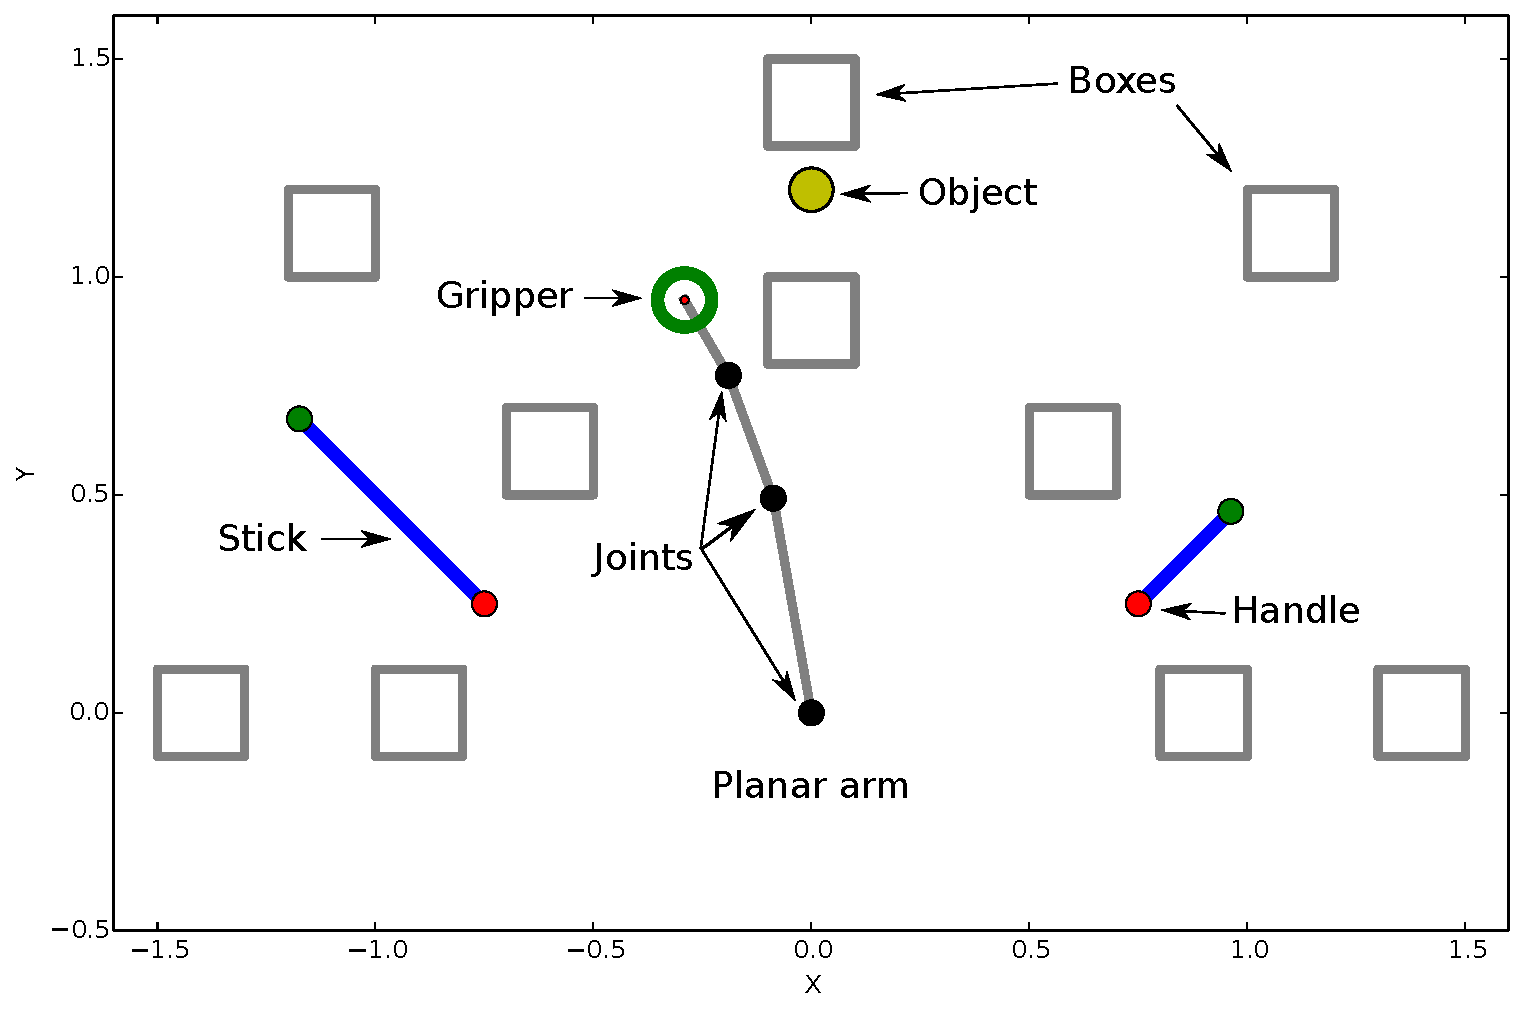
\includegraphics[width=9.12cm]{./include/tools.pdf}
			\subfloat{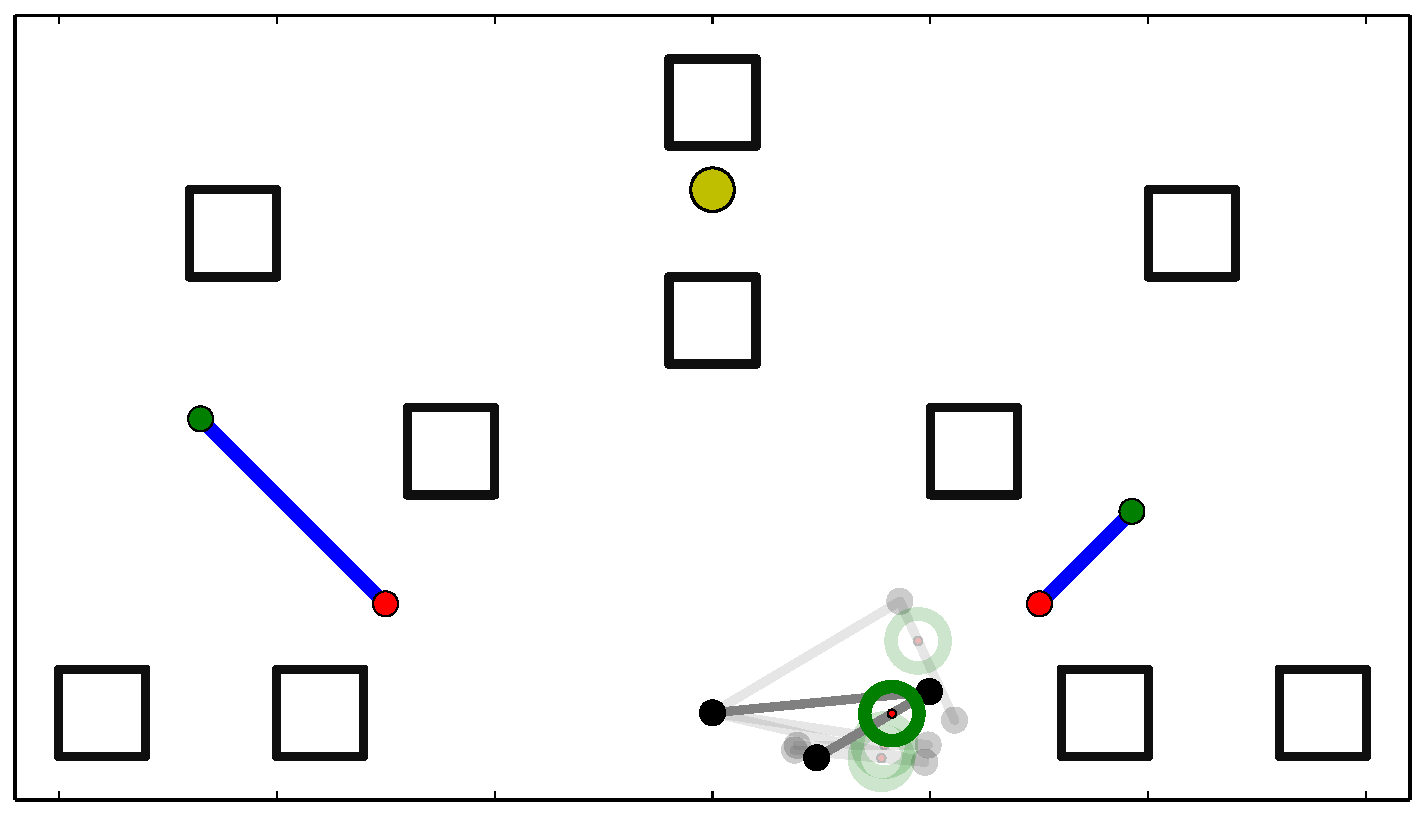
\includegraphics[width=2.8cm]{./include/mvt-16.pdf}}
			\subfloat{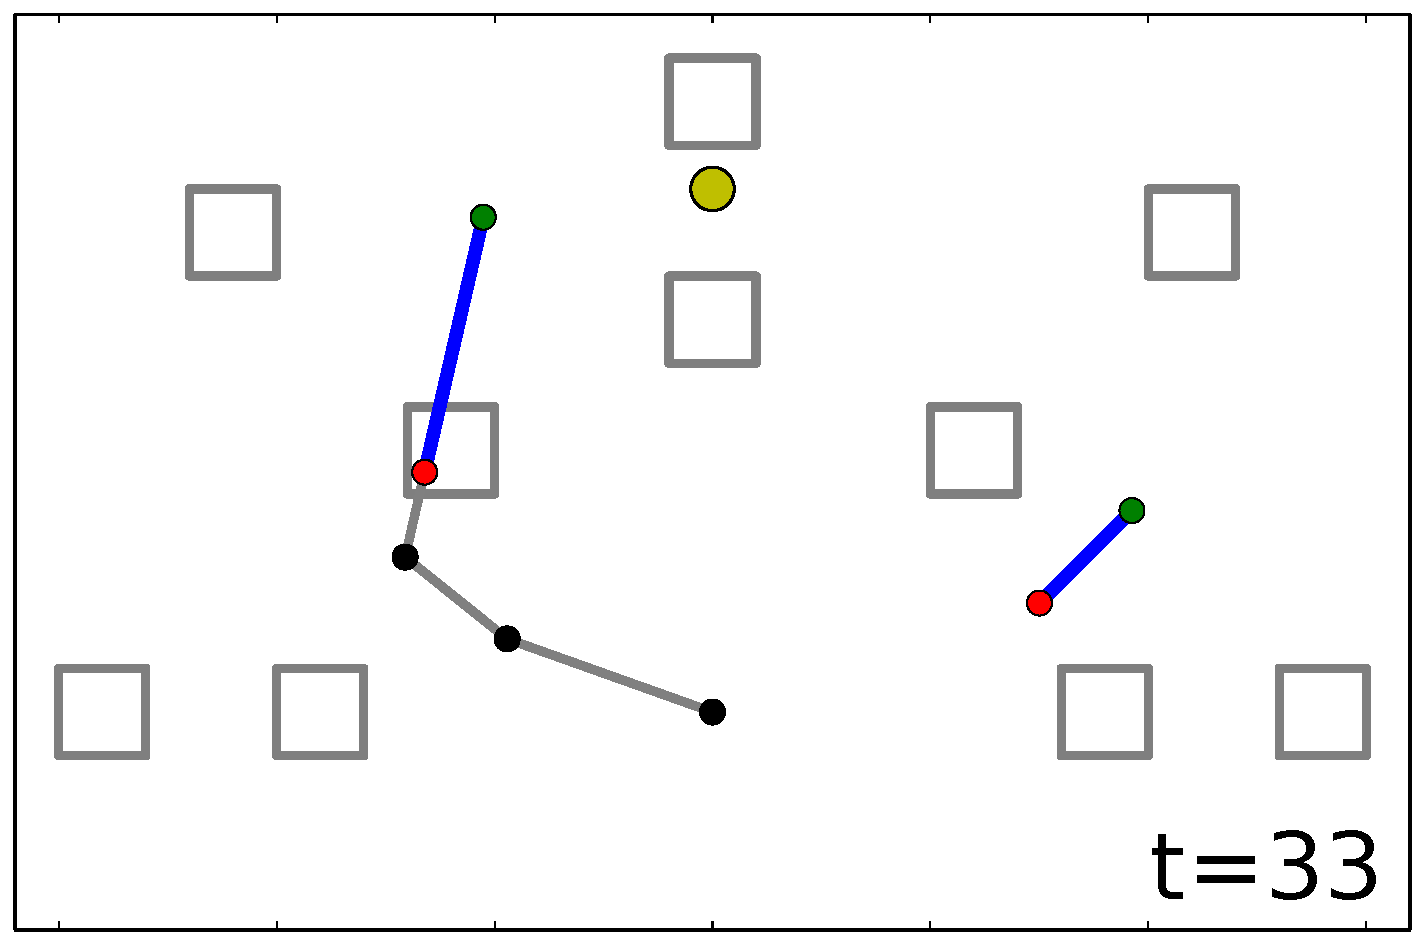
\includegraphics[width=2.8cm]{./include/mvt-32.pdf}}
			\subfloat{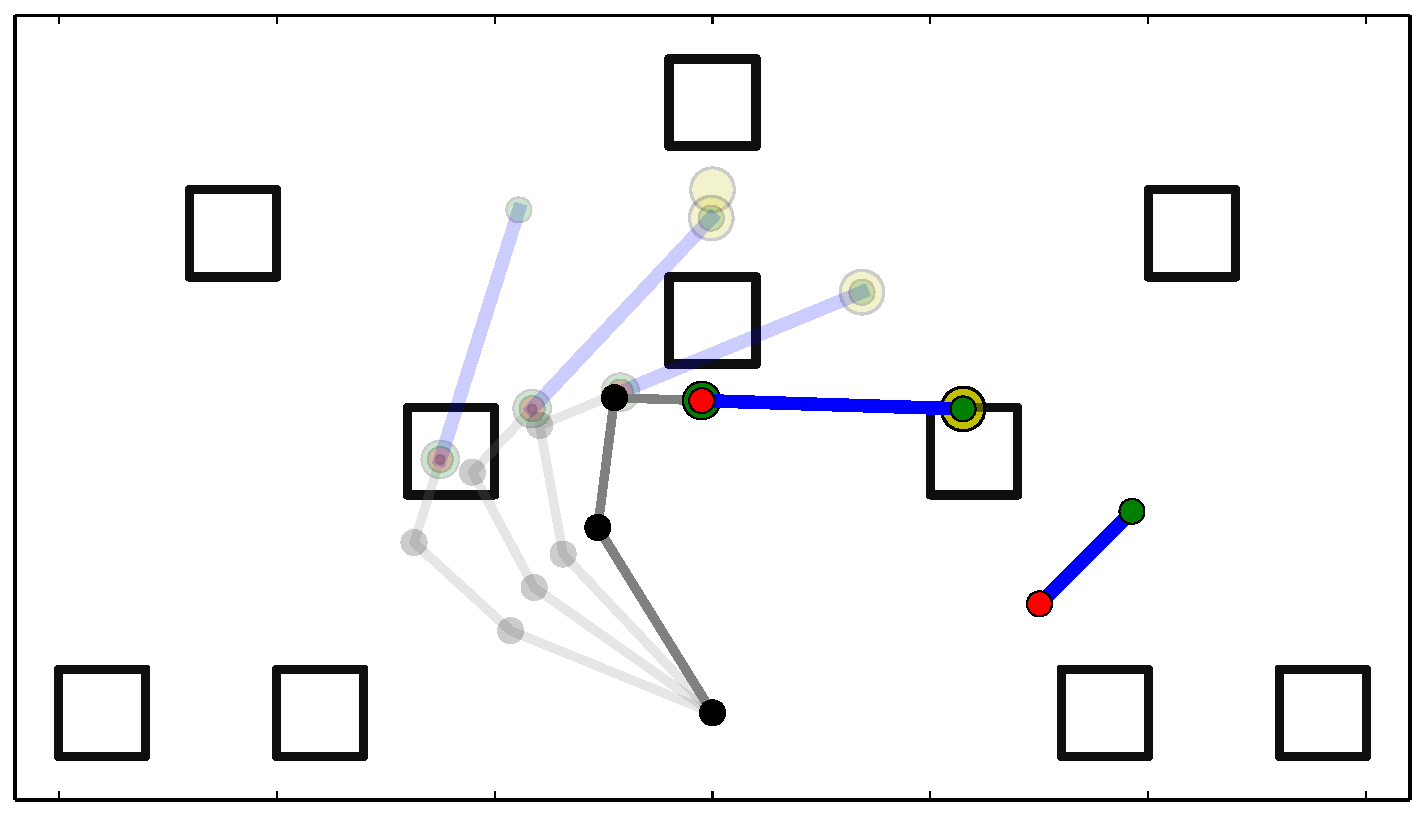
\includegraphics[width=2.8cm]{./include/mvt-49.pdf}}\\
			\hspace{-0.42cm}
			\subfloat{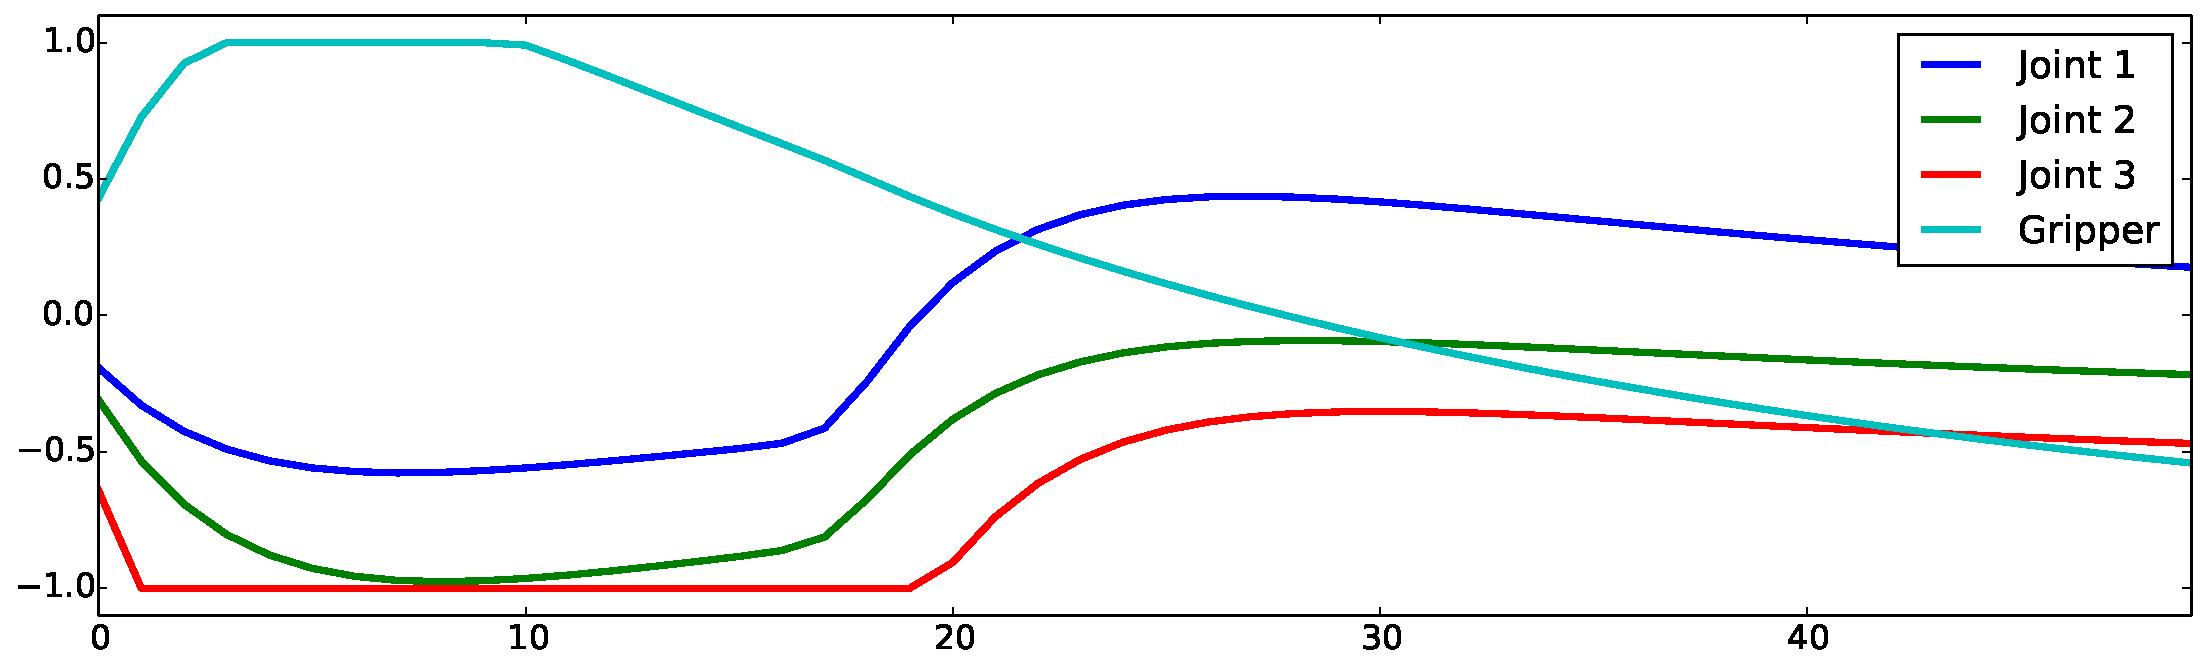
\includegraphics[width=8.8cm]{./include/dmp.pdf}}
			\caption{Top: a state of the environment. Middle: position of the arm at time steps $17$, $33$ and $50$ along the $50$ steps movement. Bottom: value of the four DMPs during the movement.}
			\label{env}
		\end{figure}

		\subsubsection{Robotic arm}
		
			The 2D robotic arm has $3$ joints plus a gripper located at the end-effector.
			Each joint can rotate from $-\pi~rad$ to $\pi~rad$ around its resting position, mapped to a standard interval of $[-1,1]$.
			The length of the $3$ segments of the arm are $0.5$, $0.3$ and $0.2$ so the total length of the arm is $1$ unit.
			The resting position of the arm is vertical with each joint at $0~rad$ and its base is fixed at position $[0, 0]$.
			The gripper $g$ has 2 possible positions: \textit{open} ($g \geq 0$) and \textit{closed} ($g < 0$) and its resting position is \textit{open} (with $g = 0$).
			The robotic arm thus has 4 degrees of freedom represented by a vector in $[-1,1]^4$.
			A trajectory of the arm will be represented as a sequence of such vectors.
		
		%
		
		\subsubsection{Motor control}
		
			We use Dynamical Movement Primitive \cite{ijspeert_dynamical_2013} to control the arm's movement as this framework permits the production of a diversity of arm's trajectories with few parameters.
			Each of the $4$ arm's degrees-of-freedom (DOF) is controlled by a DMP with a starting and a goal position equal to the rest position of the joint.
			Each DMP is parameterized by one weight on each of $3$ basis functions whose centers are distributed homogeneously throughout the movement duration.
			The weights are bounded in the interval $[-200,200]$ (mapped to the standard interval $[-1,1]$) which allow each joint to fairly cover the interval $[-1,1]$ during the movement.
			Each DMP outputs a series of $50$ positions that represents a sampling of the trajectory of one joint during the movement.		
			The arm's movement is thus parameterized by $12$ weights which are represented by the motor space $M=[-1,1]^{12}$.\\
		
		%
			
		\subsubsection{Objects and tools}
			
			A yellow sphere can be moved into one of ten fixed squared boxes. 
			The initial position of the sphere is $(0, 1.2)$ and is thus unreachable directly with the gripper.
			Two sticks can be grasped in order to reach the object.
			A small stick of length $0.3$ is located at position $(0.75, 0.25)$ with initial angle $\frac{\pi}{4}$ from the horizontal line.
			A long stick of length $0.6$ is located at position $(-0.75, 0.25)$ with initial angle $\frac{3\pi}{4}$ as in Fig. \ref{env}.			
			If the gripper is closed near the handle of one stick (closer than $0.2$), it is considered grasped and will follow the gripper's position and the angle of the arm's last segment until the gripper opens.			
			Similarly, if the other end of a stick reaches the sphere (within $0.1$), the sphere will follow the end of the stick.
			The ten boxes (identified from $1$ to $10$) are static and have size $0.2$.
			Boxes $1$ to $5$ can only be reached with the long stick, and the other five boxes can be reached with both sticks.
			At the end of the mouvement, the object is considered to be in one of the box if its center is in the box.
		
		%
		
		\subsubsection{Sensory feedback}
		
			At the end of the movement, the robot gets sensory feedback from the different items of the environment.
			It gets the trajectory of the gripper ($S_{Hand}$), the trajectory of the end of the sticks ($S_{Stick_1}$ and $S_{Stick_2}$), 
			the position of the object at the end of the mouvement ($S_{Object}$), and whether the object is in a box at the end of the mouvement and the distance between the object and the nearest box ($S_{Boxes}$).		
			The trajectory of the gripper is represented as the $x$ and $y$ positions and the aperture ($1$ or $-1$) of the gripper at $3$ time points: 
			steps $17$, $33$, $50$ during the movement of $50$ steps ($9$D).
			Similarly, the trajectories of the end points of the sticks are $3$-points sequences of $x$ and $y$ positions ($6$D for each stick).
			The agent receives the identifier (from $1$ to $10$) of the reached box if one of them has been reached by the sphere, 0 otherwise. 
			He also gets the minimal distance of the object (at the end of the movement) to the center of a box, even if none have been reached.			 
			The sensory information thus contains $9$ values for the trajectory of the gripper, $6$ for the trajectory of the end of each stick, $2$ for the end position of the object and $2$ for the boxes.
			The total sensory space $S$ has $25$ dimensions.
			
		%
		
	%
	
	\subsection{Learning architectures}

		\paragraph{}
		The problem settings for the learning agent is to explore its sensorimotor space by iteratively choosing motor parameters that represents arm trajectories and receiving sensory feedback.
		In this section we describe the different learning architectures that we will compare in the experiment.
		
		\subsubsection{Flat architectures}
			
			We define a flat architecture as directly learning a mapping between the motor space $M$ ($12$D) and the sensory space $S$ ($25$D).
			The control condition is a random motor babbling condition (F-RmB) that randomly chooses new motor parameters $m$ to try at each iteration.
			In the other conditions, the agent performs Goal Babbling, by self-generating a goal in the sensory space at each iteration and trying to reach it.
			To do so, the agent needs a sensorimotor model that learns the mapping and provides inverse inference of a probable $m$ to reach a given $s$.
			The sensorimotor model stores new information of the form ($m, s$) with $m \in M$ being the experimented motor parameters and $s \in S$ the associated sensory feedback. 
			It computes the inverse inference with the nearest neighbor algorithm: 
			it gets the motor part of the nearest neighbor of the given $s$ in $S$, and adds exploration noise (gaussian with $\sigma=0.01$) to allow new motor parameters to be explored.
			
			The agent also needs an interest model that chooses goals in the sensory space.
			To generate those goals, different strategies have been studied \cite{baranes_active_2013}. 
			It was shown that estimating the learning progress in different regions of the sensory space and generating the goals where the progress is high leads to a fast learning.
			However, this idea can't be applied in a $25$D sensory space as a learning progress signal can't be properly estimated in this volume.
			Thus we use a simpler random generation of goals in the sensory space as an interest model in the flat random goal babbling condition (F-RGB).
			We use the Explauto autonomous exploration library \cite{moulin-frier_explauto:_2014} to easily define those sensorimotor and interest models.
			
			\begin{figure}[t]
				\center
				
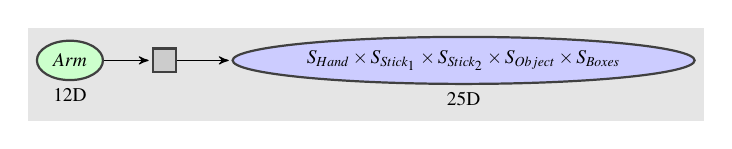
\begin{tikzpicture}[node distance=1.2cm,>=stealth',bend angle=45,auto]

	\tikzstyle{dom}   = [ellipse, thick, draw=black!75, fill=blue!20,  minimum height=4mm, minimum width=4mm]
	\tikzstyle{prim dom}   = [dom,  minimum height=5mm, minimum width=5mm,  fill=green!20]
	\tikzstyle{mod} = [rectangle, thick, draw=black!75, fill=black!20, minimum size=3mm]

	\begin{scope}[local bounding box=bb]
		\scriptsize
		\node [prim dom, label=below:$12$D] (pd1) {$Arm$};

		\node [mod] (m1) [right of=pd1] {}
		edge [pre]                  (pd1);

		\node [dom] (d1) [right of=m1, xshift=2.6cm, label=below:$25$D] {$S_{Hand} \times S_{Stick_1} \times S_{Stick_2} \times S_{Object} \times S_{Boxes}$}
		edge [pre]                (m1);
		
		
	\end{scope}
	\begin{pgfonlayer}{background}
                \node  [fill=black!10,join=round,fit=(bb)] {};
	\end{pgfonlayer}
\end{tikzpicture}

				\vspace{-0.25cm}
				
% H2
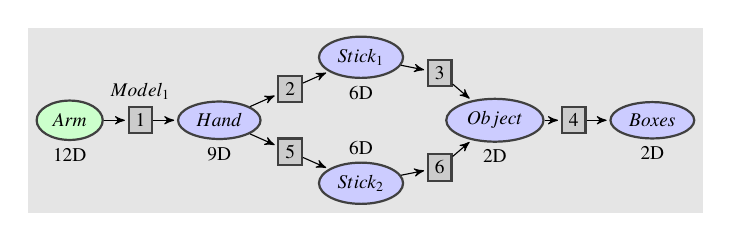
\begin{tikzpicture}[node distance=1cm,>=stealth',bend angle=45,auto]

	\tikzstyle{dom}   = [ellipse, thick, draw=black!75, fill=blue!20,  minimum height=4mm, minimum width=4mm]
	\tikzstyle{prim dom}   = [dom,  minimum height=5mm, minimum width=5mm,  fill=green!20]
	\tikzstyle{mod} = [rectangle, thick, draw=black!75, fill=black!20, minimum size=3mm]

	\begin{scope}
		\scriptsize
		\node [prim dom, label=below:$12$D] (pd1) {$Arm$};

		\node [mod, label=above:$Model_1$] (m1) [right of=pd1, xshift=-0.1cm] {$1$}
		edge [pre]                  (pd1);

		\node [dom, label=below:$9$D] (d1) [right of=m1] {$Hand$}
		edge [pre]                (m1);
		
		\node [mod] (m3) [right of=d1, xshift=-0.1cm,yshift=0.4cm] {$2$}
		edge [pre]                  (d1);
		
		\node [dom, label=below:$6$D] (d3) [right of=m3, xshift=-0.1cm,yshift=0.4cm] {$Stick_1$}
		edge [pre]                (m3);
		
		\node [mod] (m6) [right of=d1, xshift=-0.1cm,yshift=-0.4cm] {$5$}
		edge [pre]                  (d1);
		
		\node [dom, label=above:$6$D] (d6) [right of=m6, xshift=-0.1cm,yshift=-0.4cm] {$Stick_2$}
		edge [pre]                (m6);
		
		\node [mod] (m7) [right of=d6,yshift=0.2cm] {$6$}
		edge [pre]                  (d6);
		
		\node [mod] (m4) [right of=d3,yshift=-0.2cm] {$3$}
		edge [pre]                  (d3);
		
		\node [dom, label=below:$2$D] (d4) [right of=m4, xshift=-0.3cm,yshift=-0.6cm] {$Object$}
		edge [pre]                (m4)
		edge [pre]                (m7);
		
		\node [mod] (m5) [right of=d4] {$4$}
		edge [pre]                  (d4);
		
		\node [dom, label=below:$2$D] (d5) [right of=m5] {$Boxes$}
		edge [pre]                (m5);
		
		
	\end{scope}
	\begin{pgfonlayer}{background}
		\filldraw [line width=2mm,black!10]
		(d3.north  -| d5.east)  rectangle (d6.south  -| pd1.west);
	\end{pgfonlayer}
\end{tikzpicture}

				\vspace{-0.5cm}
				\caption{Architectures. Top: Flat. Bottom: Hierarchical.}
				\label{Architectures}					
			\end{figure}
				
		%
		
		\subsubsection{Hierarchical architectures}
			
			We present here an architecture that represents sensorimotor information with a hierarchical structure in Fig. \ref{Architectures}.
			
			Only the motor module (mod1) adds exploration noise ($\sigma=0.02$) even in hierarchical architecture. 
			That was the key to have more efficient hierarchical exploration. 
			Indeed, if all modules successively add exploration noise, few iterations succeed in touching the object. 
			Alternatively, if the exploration noise is reduced, exploration is less efficient as in NN only the motor module will finally apply noise on known motor commands. 
			With regression instead of NN, noise can instead be put only on the babbling module.
			
			How competence and interest of modules is computed.
			The learning progress is here computed as the absolute derivative of the reaching competence. 
			This competence associated to a sensory goal is minus the distance between the goal and the sensory point.
			
			
			\begin{itemize}
			
				\item H-RGB-RMB: Hierarchical architecture with Random Goal Babbling in each module, and Random Module Babbling. 
				Choice of tool to use based on the maximum competence of the two modules to reach the goal object point.
				\item H-RGB-P-AMB: same as H-RGB-RMB but Active Module Babbling with a choice of module to babble Proportional to interest of modules  ($\epsilon$-prop: probabilities proportional to interest but with $\epsilon=10\%$ of random choice). 
				\item H-RGB-GR-AMB: same as H-RGB-P-AMB but the choice of module to babble is $\epsilon$-greedy with $\epsilon=0.1$
				\item H-RGB-P-AMB-PGITC: same as H-RGB-P-AMB but the choice of the tool to use is Proportional to the Global Interest of the two modules ($\epsilon$-prop).

			\end{itemize}
				
				
		%
		Nearest Neighbors, $100$ iterations of Motor babbling and then $100000$ iterations of the condition. $100$ trials per condition.
		
		
		



	%
	
	\subsection{Measures}
		
		
		We provide a measure of the different types of behaviors with the sticks and the object during exploration. 
		We categorize the behaviors into three types.
		In the first category ($hand$) are mouvements of the arm that did not grab any stick and thus not moved the out-of-reached object.
		The second category ($stick$) are mouvements that did grab one of the two sticks but did not touch the object with it.
		The third category ($object$) contains the mouvements where both a stick was grabbed and the object was moved by the stick.
		
		Also, for each condition we measure the total exploration of the different sensory spaces during training. 
		The exploration of the hand, sticks and object spaces is defined as the number of reached cells 
		in a $100\times100$ discretization of the (X,Y) space of the position at timestep $50$ (end of movement).
		The exploration of the boxes is the number of boxes that have been filled with the object during training.
			
	%
	
%


\section{Results}
	

	\paragraph{}
	Fig. \ref{res_interests} shows details about one trial of the condition H-RGB-P-AMB. 
	We can see the interest of each module during the whole experiment.
	The interests of modules 2 and 5 increase abruptly once the arm succeeded in grabbing the corresponding stick.
	Following that, the interests of modules 3 and 6 also increase abruptly when the object has been touched by the corresponding stick.
	An exemple of exploration of the $2$D space with the object is also provided in Fig. \ref{res_interests}(b) corresponding to the same condition.
	
	\begin{figure*}[ht]
		\centering
		\subfloat[]{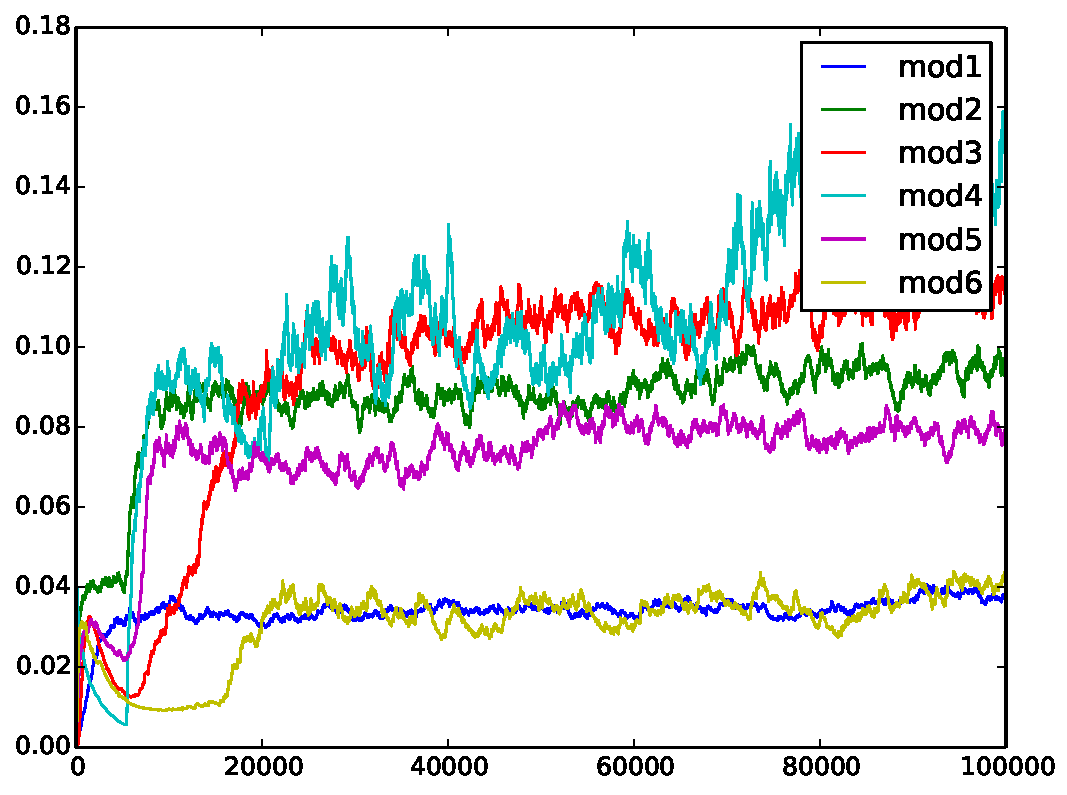
\includegraphics[width=9cm]{./include/H-RGB-P-AMB-log9-interests-100000.pdf}}
		\subfloat[]{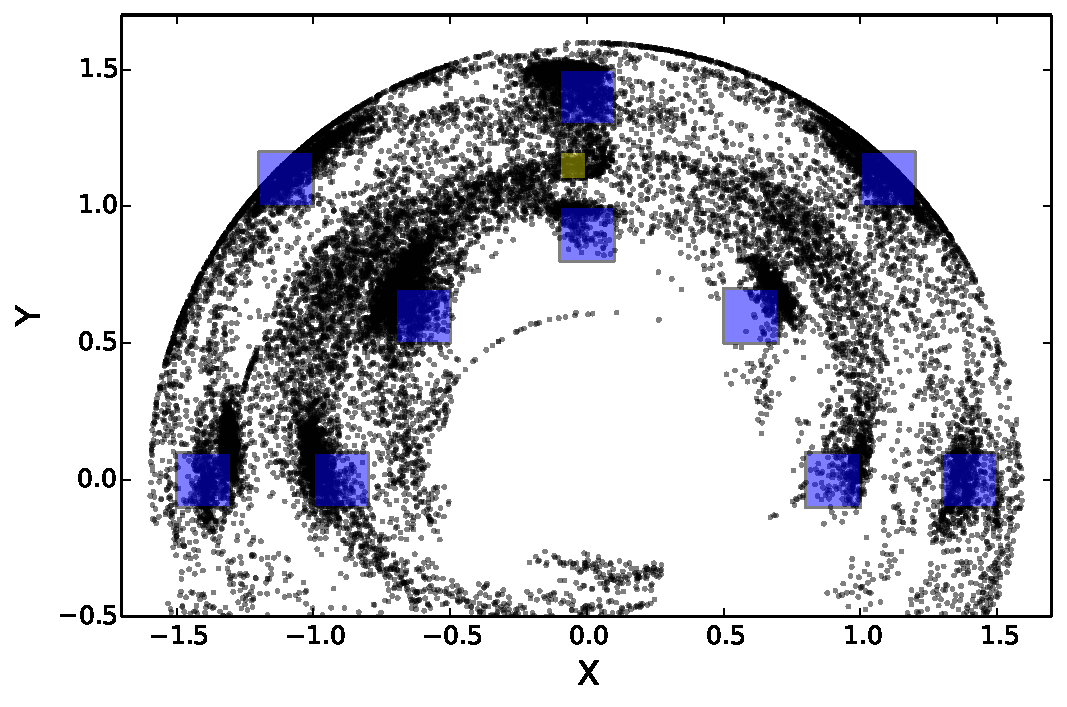
\includegraphics[width=9cm]{./include/H-RGB-P-AMB-log9-obj-explo.pdf}}
		\caption{Condition H-RGB-P-AMB. (a) Interests of each module. (b) Exploration of the object space: each dot is one point reached with the object at the end of one movement.}
		\label{res_interests}
	\end{figure*}


	\paragraph{}
	Fig. \ref{res_ow} shows the proportion of the three categories of behavior along the $100000$ iterations for conditions H-RGB-GR-AMB and H-RGB-P-AMB.

	\begin{figure*}[ht]
		\centering
		\subfloat[H-RGB-GR-AMB]{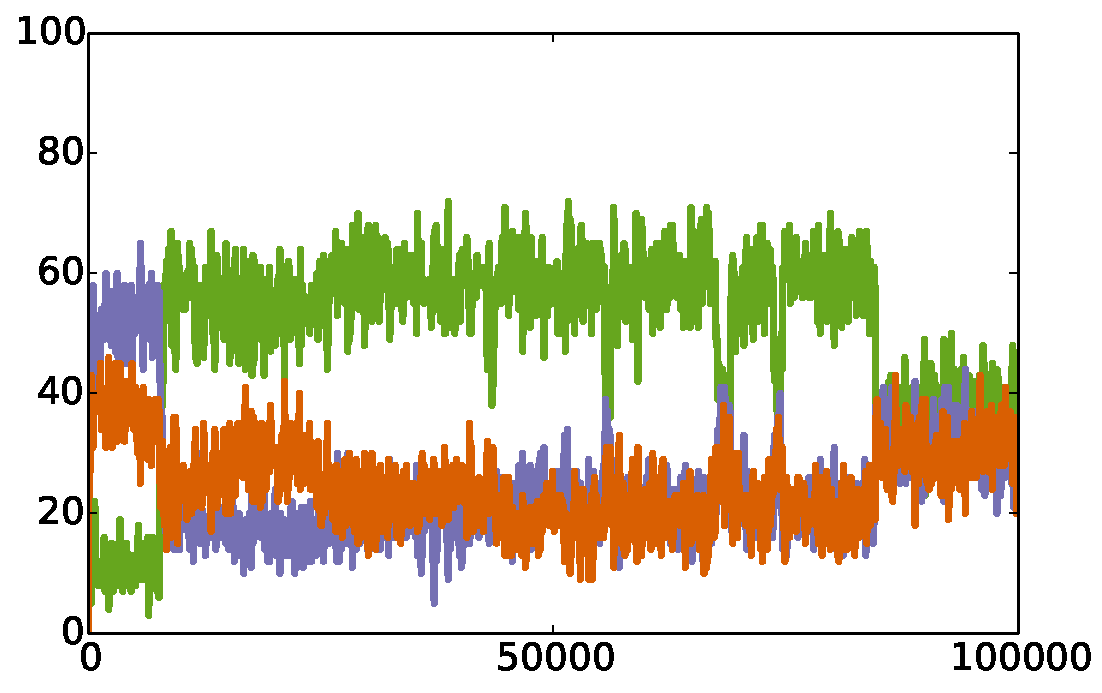
\includegraphics[width=8cm]{./include/H-RGB-GR-AMB-log15-events-100000.pdf}}
		\subfloat[H-RGB-P-AMB]{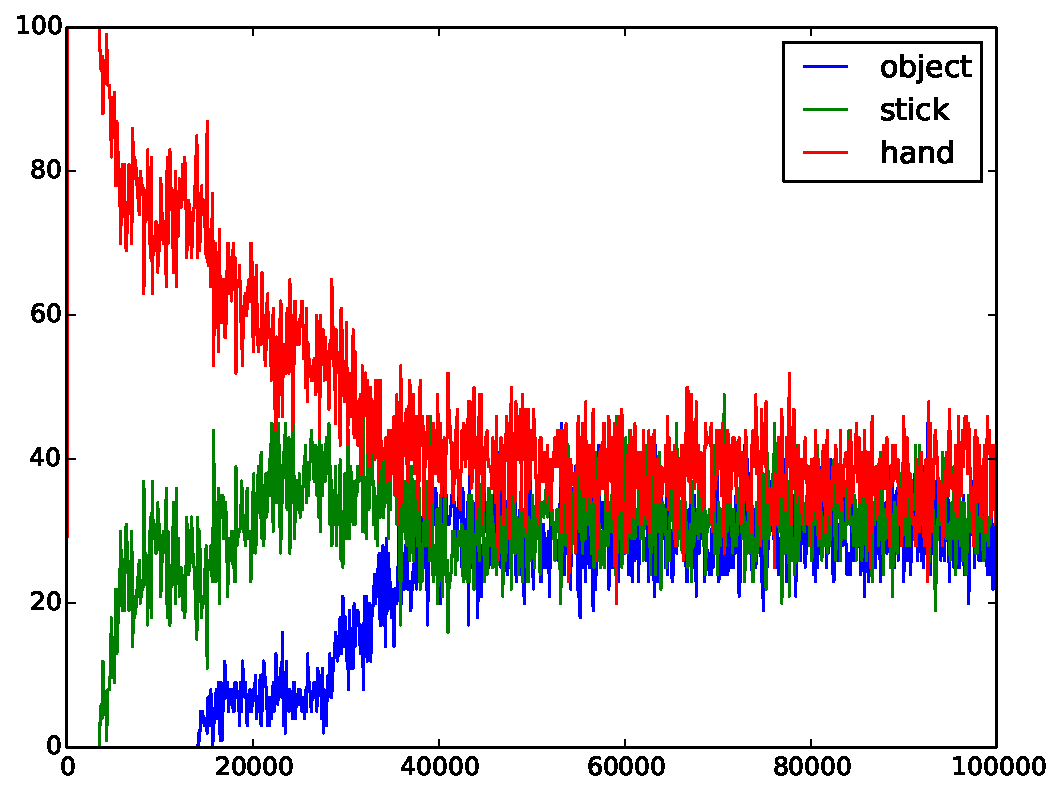
\includegraphics[width=8cm]{./include/H-RGB-P-AMB-log8-events-100000.pdf}}
		\caption{Behavioral measure}
		\label{res_ow}
	\end{figure*}
	
	\begin{figure}[ht]
		\centering
		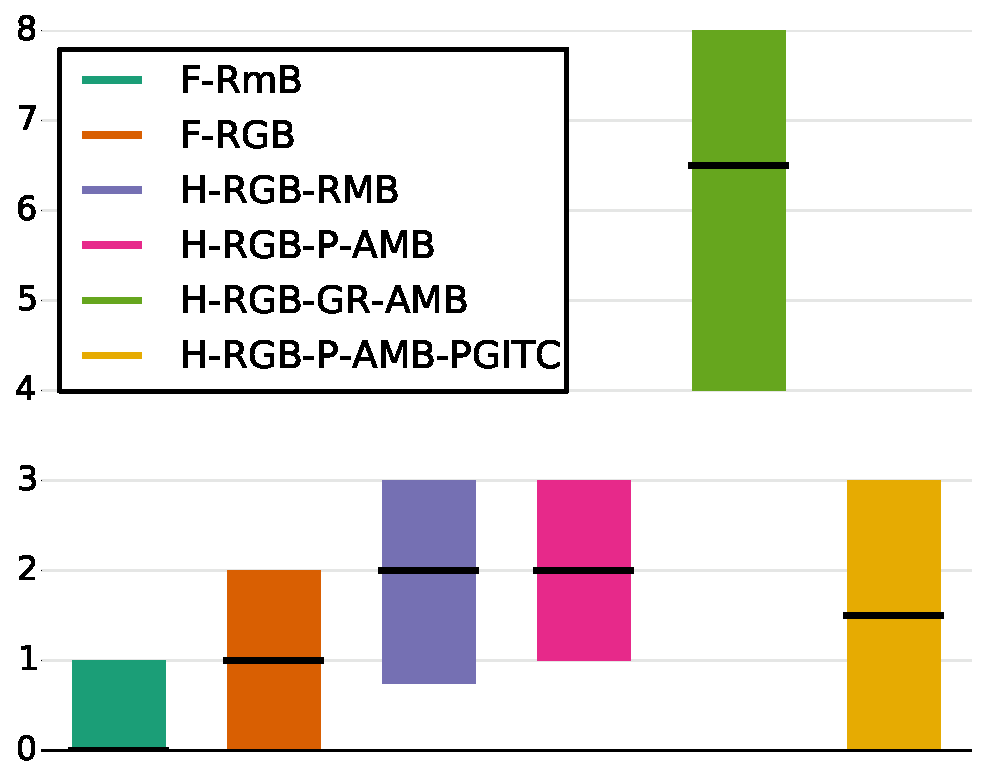
\includegraphics[width=7cm]{./include/nbc.pdf}
		\caption{Number of abrupt behavioral changes}
		\label{res_nbc}
	\end{figure}


	\paragraph{}
	Fig. \ref{res_explo} shows the total exploration of the different sensory spaces for each condition.
	We provide statistical Mann-Whitney U test results of comparisons of the exploration at the end of the experiments in different pairs of conditions.
	Firstly, the Motor Babbling condition (F-RmB) have more explored $S_{Hand}$ and less $S_{Object}$ and $S_{Boxes}$ compared to the other conditions ($p<0.0001$).
	Then, F-RGB explores all spaces less than H-RGB-RMB condition ($p<0.01$).
	Also, H-RGB-GR-AMB shows lower exploration all spaces than H-RGB-P-AMB ($p<0.01$).
	Condition H-RGB-P-AMB-PGITC explores more $S_{Stick_2}$ ($p<0.05$) than condition H-RGB-P-AMB, and difference is not significant in other spaces.
	
	\begin{figure*}[ht]
		\centering
		
\includegraphics[width=14cm]{./include/xp1-explo-legend.pdf}\\
		\vspace{-0.3cm}
		\subfloat[$Hand$]{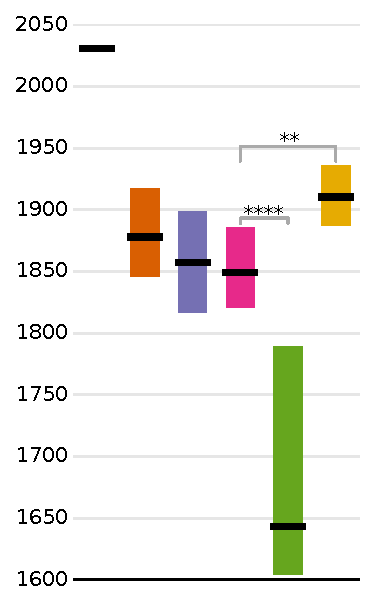
\includegraphics[width=3.5cm]{./include/xp1-explo-hand.pdf}}
		\subfloat[$Stick_1$]{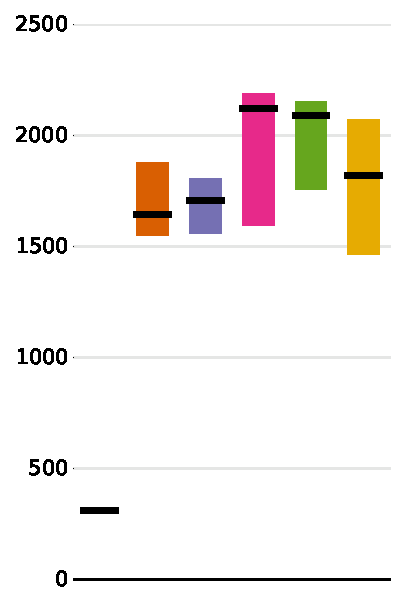
\includegraphics[width=3.5cm]{./include/xp1-explo-stick_1.pdf}}
		\subfloat[$Stick_2$]{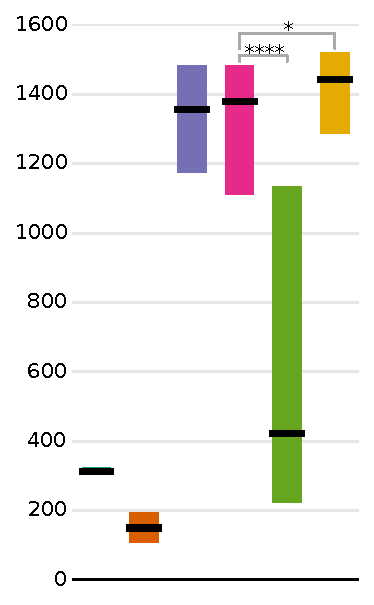
\includegraphics[width=3.5cm]{./include/xp1-explo-stick_2.pdf}}
		\subfloat[$Object$]{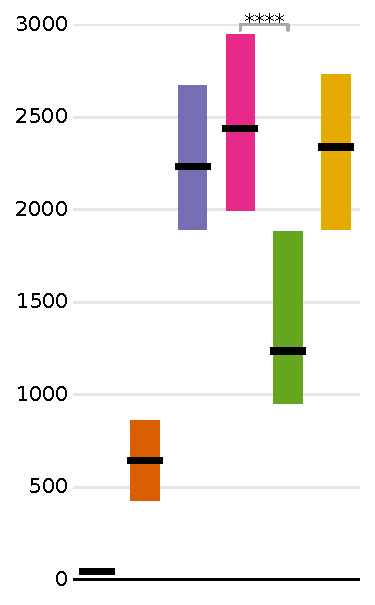
\includegraphics[width=3.5cm]{./include/xp1-explo-obj.pdf}}
		\subfloat[$Boxes$]{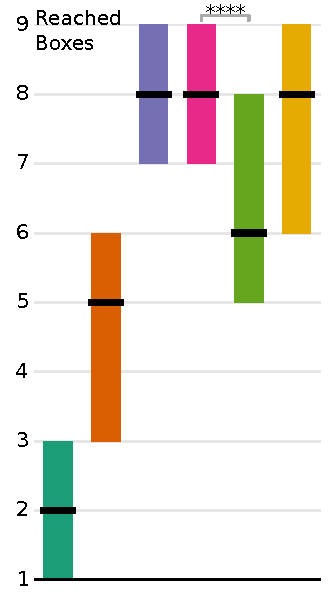
\includegraphics[width=3.5cm]{./include/xp1-explo-box.pdf}}
		\caption{Exploration of sensory spaces.}
		\label{res_explo}
	\end{figure*}


	\paragraph{}
	Fig. \ref{res_choice} shows a comparison of the choice of tool to reach a given object goal position in the conditions H-RGB-P-AMB and H-RGB-P-AMB-PGITC.
	In those conditions, module $4$ learns a mapping between $S_{Object}$ and $S_{Boxes}$. 
	When this module is babbling, it chooses a random goal $s_b \in S_{Boxes}$ and infers the best object position $s_o$ to reach $s_b$.
	To reach $s_o$, one of the tools ($Stick_1$ with module $3$ or $Stick_2$ with module $6$) is chosen. 
	We plot all those choices, at position $s_o$ on a $2$D space, with color blue if $Stick_1$ was chosen and red if $Stick_2$ was chosen, in one figure for each of the two conditions.
	We can see two very different choice structures.
	However, goal that can be reached with both tools are more often chosen to be explored with the long stick in the interest-based choice of condition H1 than in competence-based choice of condition H1-CL.
	
	\begin{figure*}[ht]
		\subfloat[H-RGB-P-AMB]{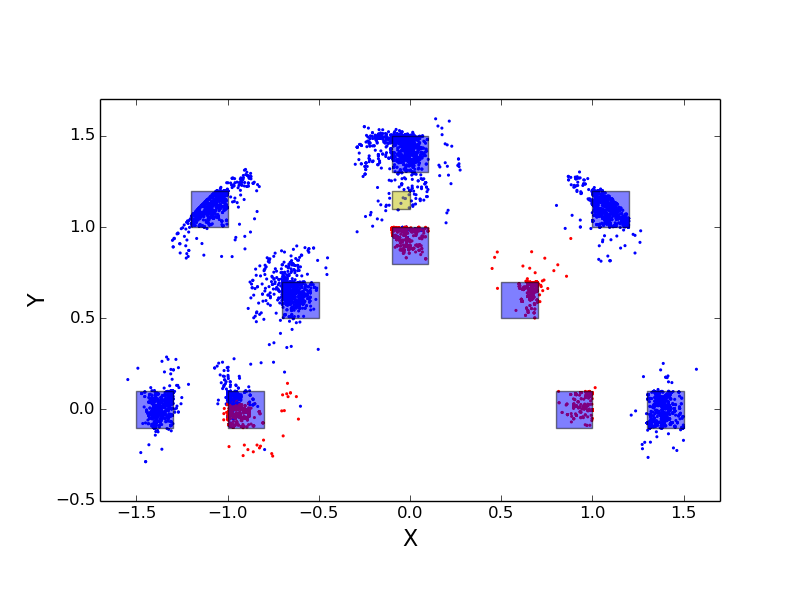
\includegraphics[width=9cm]{./include/H-RGB-P-AMB-log9-choice_mod4.png}}
		\subfloat[H-RGB-P-AMB-PGITC]{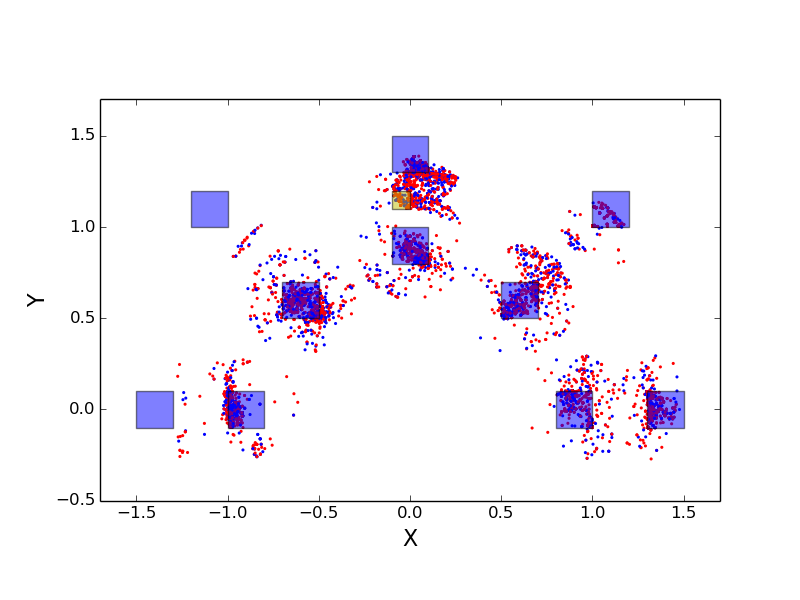
\includegraphics[width=8.8cm]{./include/H-RGB-P-AMB-PGITC-log3-choice_mod4.png}}
		\caption{Chosen tool depending on object goal position. Blue points: long stick choice. Red points: small stick choice.}
		\label{res_choice}
	\end{figure*}
	
%


\section{Discussion}

	\subsection{F-AGB vs H-RGB-P-AMB vs H-RGB-GR-AMB}
	
	
	%
	
	\subsection{H-RGB-P-AMB vs H-RGB-P-AMB-PGITC}
	
	
	%
	
%


\section{Conclusion}

%


\section{Acknowledgments}

%




\bibliographystyle{apacite}

\setlength{\bibleftmargin}{.125in}
\setlength{\bibindent}{-\bibleftmargin}

\bibliography{include/bibliography}


\end{document}
